\documentclass[11pt]{article}
\usepackage[margin=1in]{geometry}
\usepackage[T1]{fontenc}
\usepackage{lmodern}
\usepackage{microtype}
\usepackage{amsmath}
\usepackage{booktabs}
\usepackage{tabularx}
\usepackage{xcolor}
\usepackage{tikz}
\usetikzlibrary{arrows.meta,positioning,fit}
\usepackage[numbers,sort&compress]{natbib}
\usepackage[hidelinks]{hyperref}
\usepackage{url}

\newcommand{\pending}[1]{\textcolor{red}{[#1]}}
\newcolumntype{Y}{>{\raggedright\arraybackslash}X}

\title{Serving Telemetry for Local LLM Inference:\\
What Production Systems Measure, and How to Recover It from llama.cpp}
\author{Luiz Henrique Sim\~oes\\ \small Independent researcher \\ \small\texttt{luizhenriquesimoes@usp.br} \textperiodcentered{} \texttt{simoeshz@gmail.com}}
\date{September 2026 (deployment description revised 21 September) \\ \small Technical note. Not peer reviewed.}

\begin{document}
\maketitle

\begin{abstract}
Production LLM serving systems, their open standards and the serving literature share one
vocabulary of metrics: time to first token timed from request arrival, queue time separate from
prefill, per-gap inter-token latency distinct from mean time per output token, goodput as
\emph{joint} SLO attainment, current KV-cache occupancy, speculative-decoding acceptance and mean
acceptance length, and energy integrated from hardware counters rather than sampled power. This note
synthesises those definitions from 16 arXiv papers and 25 specifications, engine documents and
source files, all opened during the research. It then applies them to a single-host llama.cpp
deployment serving a 27B-parameter reasoning model at a 262,144-token context on two 16\,GB consumer
GPUs. llama.cpp natively exposes 16 serving series and no latency histogram. It records no request
arrival time, so queue time, arrival-based TTFT, inter-token gaps, HTTP errors and finish reasons are
unobservable from the server alone. A first deployment built from the server log shows how easily
the definitions drift: 4 of its 7 derived rules that were checked never returned a value, and its
``TTFT'' was prefill time. We describe the adapted stack: a transparent measuring proxy, a server
sidecar, an NVML exporter using the GPU performance-monitoring interface on consumer cards, and
provisioned dashboards. Each metric is mapped to the standard it follows.
\end{abstract}

\section{Introduction}

A serving engine can be tuned only against what is measured, and what is measured depends on
definitions that differ more than their shared names suggest. ``Time to first token'' starts at
request arrival in OpenTelemetry~\citep{otel_genai_metrics} and vLLM~\citep{vllm_metrics}. The
llama.cpp server log starts the same clock only when a slot begins prompt
processing~\citep{llamacpp_server}. With a single decoding slot, the difference is the entire wait
behind the previous request.

This note accompanies a measurement study of quantization, context length and speculative decoding
for Qwen3.8-27B on consumer hardware~\citep{simoes2026benchmarks}. The study's host serves that model
continuously from a llama.cpp server with a 262,144-token window, one slot, and reasoning enabled by
default. The host has two 16\,GB consumer GPUs with no GPU interconnect, so the model is split
layer-wise across both cards. Host memory is smaller than the model file.

Two served configurations appear in this note. The telemetry was built and verified on 14 September
2026 against the first: a 6-bit GGUF build (UD-Q6\_K), a 4-bit (q4\_0) KV cache, and the model's
built-in multi-token-prediction (MTP) drafter with two draft tokens. Since 19 September the host
serves the configuration the study selected: a 4-bit build (UD-Q4\_K\_XL), an 8-bit (q8\_0) KV cache,
and a separate block-diffusion drafter (DFlash2) with seven draft tokens, on a newer upstream
llama.cpp build. Nothing in the design depends on which of the two is running; Section~\ref{sec:update}
records what was re-checked after the change. All verification figures in Section~\ref{sec:verification}
are from the first configuration and are labelled as such.

This note records three things:
\begin{enumerate}
\item How production engines, open standards and the serving literature define serving telemetry.
\item What llama.cpp exposes against that taxonomy.
\item How the definitions were adapted for this deployment, including the defects a first,
log-based attempt contained.
\end{enumerate}

\paragraph{Method.} Three parallel research passes each covered one area: (A) the llama.cpp
telemetry surface; (B) serving standards, engine metric catalogues and the serving literature; and
(C) hardware, energy, host and output-behaviour telemetry together with monitoring method. Each pass
opened its sources and marked every source either as fetched or as recalled. Only fetched sources
are cited here. arXiv metadata was re-checked against the arXiv API. Claims about the running
server were checked read-only against the live endpoints and the engine source.

\section{How serving telemetry is defined}

\subsection{Latency is decomposed at request boundaries}

\paragraph{TTFT.} Every standard examined times the first token from request arrival or send, so
queueing is included:
\begin{itemize}
\item vLLM's \texttt{time\_to\_first\_token\_seconds} starts at frontend arrival~\citep{vllm_metrics};
\item OpenTelemetry's \texttt{gen\_ai.server.time\_to\_first\_token} is described as covering ``the
time spent in the queue and the prefill phase''~\citep{otel_genai_metrics};
\item NVIDIA AIPerf times from request start~\citep{nvidia_aiperf};
\item MLPerf Inference judges TTFT per query at a latency percentile~\citep{mlperf_rules}.
\end{itemize}

\paragraph{Queue and prefill.} vLLM separates queue time (queued $\to$ scheduled) from prefill time
(scheduled $\to$ first token)~\citep{vllm_metrics}, and TGI exports a queue-duration
histogram~\citep{tgi_metrics}.

\paragraph{Decode.} Two quantities are distinguished:
\begin{itemize}
\item \emph{Time per output token} (TPOT) is a per-request mean, the decode time divided by
$n_\text{out}-1$ (OpenTelemetry, vLLM, MLPerf).
\item \emph{Inter-token latency} (ITL) records one observation per gap between emitted tokens or
chunks (vLLM, NVIDIA Dynamo~\citep{nvidia_dynamo}, AIPerf).
\end{itemize}
The distinction matters under speculative decoding, where tokens arrive in bursts: a mean TPOT hides
a bimodal gap distribution.

\paragraph{Reasoning models.} For reasoning models AIPerf adds time to first \emph{output}
(non-reasoning) token~\citep{nvidia_aiperf}. OpenAI's API reports reasoning tokens separately, and
documents responses that end before any visible output~\citep{openai_reasoning}.

\paragraph{Streaming experience.} Etalon's fluidity-index~\citep{agrawal2024etalon} and Andes'
quality-of-experience metric~\citep{liu2024andes} score the timeline of token delivery rather than
single percentiles.

\subsection{Goodput is joint SLO attainment}

DistServe defines SLO attainment as the proportion of requests that meet their SLOs, and goodput as
the highest request rate served at a target attainment~\citep{zhong2024distserve}. AIPerf reports
goodput as good requests per second~\citep{nvidia_aiperf}. In both, a request is judged against
\emph{all} its objectives at once. Sarathi-Serve frames the throughput--latency trade-off that
goodput is meant to expose~\citep{agrawal2024sarathi}. Splitwise~\citep{patel2023splitwise} and
DistServe both motivate recording prefill and decode as separate phases.

\subsection{Saturation is the queue, the running set and the KV cache}

The Kubernetes Gateway API Inference Extension specifies the load-balancing contract a model server
must export. It has three gauges: queued requests, running requests and KV-cache
utilisation~\citep{gie_msp}. vLLM and SGLang map these to their own metric
names~\citep{vllm_metrics,sglang_metrics}.

Beyond that contract:
\begin{itemize}
\item \textbf{KV-cache occupancy.} PagedAttention made occupancy the central memory
quantity~\citep{kwon2023pagedattention}.
\item \textbf{Prefix-cache hits.} These are counted in tokens, as hits over queries, by vLLM and
SGLang~\citep{vllm_metrics,sglang_metrics}. They are the dominant variable for KV-centric designs
such as Mooncake~\citep{qin2024mooncake}.
\item \textbf{Scheduling.} Llumnix treats queueing and migration as the levers~\citep{sun2024llumnix}.
\end{itemize}

\subsection{Speculative decoding has three quantities, not one}

Three quantities are distinguished:
\begin{itemize}
\item \textbf{Acceptance rate}, accepted draft tokens over drafted tokens.
\item \textbf{Per-token acceptance probability $\alpha$}, from which the expected tokens per step
follow as $(1-\alpha^{\gamma+1})/(1-\alpha)$ for draft length $\gamma$~\citep{leviathan2023spec}.
\item \textbf{Mean acceptance length}, $\tau = 1 + \text{accepted}/\text{drafts}$, the quantity
EAGLE reports~\citep{li2024eagle} and vLLM computes~\citep{vllm_metrics}.
\end{itemize}
Per-position acceptance counters give the conditional $\alpha_k$, which separates a drafter failure
from an effect of position. Wall-clock speedup requires a paired no-speculation
baseline~\citep{leviathan2023spec,chen2023specsampling,cai2024medusa}.

\subsection{Hardware utilisation and energy need the right instrument}

\paragraph{Utilisation.} NVML's classic utilisation is the fraction of the sample period during which
\emph{at least one} kernel ran~\citep{nvml_api}. DCGM's profiling metrics instead report
streaming-multiprocessor activity and occupancy, memory-bandwidth activity and PCIe
throughput~\citep{dcgm_features}.

\paragraph{Energy.} Energy should come from the cumulative counter, not from integrated power
samples:
\begin{itemize}
\item \texttt{nvidia-smi} power readings cover only part of runtime on common data-centre GPUs, and
correcting for this materially reduces energy error~\citep{yang2023parttime}.
\item Zeus and the ML.ENERGY benchmark measure energy per request and per response from
counters~\citep{zeus_measure,chung2023bestpractices,chung2025mlenergy}.
\item The AI Energy Score normalises to Wh per 1,000 queries~\citep{aienergyscore}.
\item Google's accounting of production inference counts idle provisioned capacity as a separate
term~\citep{elsworth2025google}.
\end{itemize}

\subsection{Method: golden signals, USE, workload shape}

Three frameworks organise the dashboards. The four golden signals are latency, traffic, errors and
saturation, and they count a successful response with wrong content as an
error~\citep{sre_monitoring}. The USE method (utilisation, saturation, errors) applies per
resource~\citep{gregg_use}. Pressure-stall information quantifies host saturation~\citep{linux_psi}.

Workload traces from Azure~\citep{azure_trace} and BurstGPT~\citep{wang2024burstgpt} show which
request-shape distributions matter: input and output length, and inter-arrival burstiness.

\begin{table}[t]
\centering\small
\caption{Serving-telemetry taxonomy and the definition each family follows.}
\label{tab:taxonomy}
\begin{tabularx}{\linewidth}{@{}lYl@{}}
\toprule
family & metrics & defined by \\
\midrule
latency & TTFT (arrival), time to first answer token, queue, prefill, TPOT, ITL per gap, E2E &
\citep{otel_genai_metrics,vllm_metrics,nvidia_aiperf,mlperf_rules} \\
goodput & joint SLO attainment; good requests/s & \citep{zhong2024distserve,nvidia_aiperf} \\
saturation & queued, running, KV-cache occupancy, prefix-cache hit ratio & \citep{gie_msp,vllm_metrics,sglang_metrics} \\
speculation & acceptance rate, $\tau$, per-position $\alpha_k$ & \citep{leviathan2023spec,li2024eagle,vllm_metrics} \\
errors & HTTP class, aborts, finish reason, empty answers & \citep{sre_monitoring,otel_genai_spans,openai_reasoning} \\
request shape & ISL (incl.\ cached), OSL, reasoning tokens, requested budget & \citep{nvidia_aiperf,azure_trace,wang2024burstgpt} \\
GPU & SM activity/occupancy, memory bandwidth, PCIe, energy counter & \citep{dcgm_features,nvml_api} \\
energy & J/token and J/request from counters, idle power, Wh/1k requests & \citep{chung2025mlenergy,aienergyscore,elsworth2025google} \\
host & PSI, swap, faults, CPU package energy & \citep{gregg_use,linux_psi} \\
\bottomrule
\end{tabularx}
\end{table}

\section{What llama.cpp exposes}

The server's Prometheus endpoint exports 16 series: 10 counters, 5 gauges and one per-position
speculative-decoding counter. There are no histograms and no KV-occupancy gauge. The engine source
and its issue history~\citep{llamacpp_server,llamacpp_kv_issue} show five properties that shape
everything downstream.

\begin{enumerate}
\item \textbf{No arrival time is recorded.} The per-request clock starts when a slot begins prompt
processing, after HTTP parsing, templating, tokenisation and the deferred queue. The logged ``total
time'' is prefill plus decode.
\item \textbf{The KV-occupancy gauge was removed.} It was judged too implementation-specific to
expose, and a request to restore it has stalled~\citep{llamacpp_kv_issue}. What remains,
\texttt{n\_tokens\_max}, is a lifetime high-water mark.
\item \textbf{Two gauges reset whenever \texttt{/metrics} is read.} The throughput gauges average over
the window since the previous scrape by any reader, so any second reader corrupts them. Decode and
speculation counters advance only when a request ends.
\item \textbf{\texttt{truncated} is not \texttt{length}.} The flag is set only when the context window
fills. Exhausting \texttt{max\_tokens} yields \texttt{finish\_reason: length} with
\texttt{truncated} false.
\item \textbf{A lot is available per request, but only through the response or the slot endpoint.}
Each response carries a \texttt{timings} object (prompt, cached and decoded tokens with their
durations, drafted and accepted tokens). \texttt{/slots} reports live per-slot prompt, cache and
decode progress.
\end{enumerate}

\section{Adaptation for this deployment}

\subsection{Constraints}

Six properties of the deployment constrain the design:
\begin{itemize}
\item \textbf{One decoding slot}, so any concurrent request queues, and any synthetic probe request
delays a real one.
\item \textbf{Reasoning on by default}, so the first token is usually a reasoning token.
\item \textbf{A full-window prefill takes minutes}, so fixed TTFT SLOs are meaningless at depth.
\item \textbf{Speculative decoding emits tokens in bursts.}
\item \textbf{Consumer GPUs}: NVIDIA does not document DCGM profiling fields for them.
\item \textbf{Memory headroom is small}, which rules out tracing and log-store backends.
\end{itemize}

\subsection{Architecture}

Figure~\ref{fig:arch} shows the stack. Its five components are:
\begin{itemize}
\item \textbf{A transparent measuring proxy.} It takes over the address clients already use, and the
server moves to loopback. It relays every path byte-for-byte and streams chunk by chunk. For
inference endpoints it timestamps arrival, the first token-bearing chunk, the first answer chunk,
every chunk gap and the last byte. It parses \texttt{finish\_reason}, \texttt{usage} and the server's
\texttt{timings}, evaluates SLO classes per request, and writes one content-free JSON record per
request.
\item \textbf{A server sidecar.} It polls \texttt{/health}, \texttt{/slots} and \texttt{/props}; it
never polls \texttt{/metrics}, because of property 3. It follows the container log with wall-clock
timestamps and exports launch-configuration provenance as info labels.
\item \textbf{An NVML exporter.} It reads the cumulative energy counter, the GPU performance-monitoring
(GPM) ratios for streaming-multiprocessor utilisation, occupancy and memory bandwidth, PCIe
throughput, the PCIe replay counter, XID events and per-process memory attributed to containers.
Both consumer cards answered every one of these queries.
\item \textbf{Recording rules and alerts} following Table~\ref{tab:taxonomy}.
\item \textbf{Four provisioned dashboards}: golden signals, request anatomy, GPU and energy (USE per
card), and host.
\end{itemize}

\begin{figure}[t]
\centering
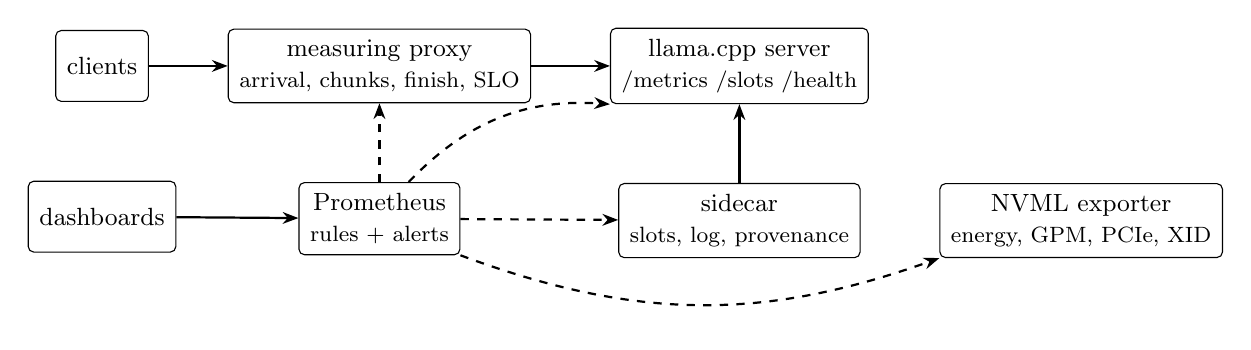
\begin{tikzpicture}[
  box/.style={draw, rounded corners=2pt, align=center, font=\small, minimum height=0.9cm, inner sep=4pt},
  arr/.style={-{Stealth[length=2mm]}, thick}]
\node[box] (client) {clients};
\node[box, right=1.0cm of client] (proxy) {measuring proxy\\\footnotesize arrival, chunks, finish, SLO};
\node[box, right=1.0cm of proxy] (server) {llama.cpp server\\\footnotesize /metrics /slots /health};
\node[box, below=1.0cm of server] (side) {sidecar\\\footnotesize slots, log, provenance};
\node[box, below=1.0cm of proxy] (prom) {Prometheus\\\footnotesize rules + alerts};
\node[box, below=1.0cm of client] (graf) {dashboards};
\node[box, right=1.0cm of side] (nvml) {NVML exporter\\\footnotesize energy, GPM, PCIe, XID};
\draw[arr] (client) -- (proxy);
\draw[arr] (proxy) -- (server);
\draw[arr] (side) -- (server);
\draw[arr, dashed] (prom) -- (proxy);
\draw[arr, dashed] (prom) -- (side);
\draw[arr, dashed] (prom.south east) to[bend right=20] (nvml.south west);
\draw[arr, dashed] (prom) to[bend left=25] (server.south west);
\draw[arr] (graf) -- (prom);
\end{tikzpicture}
\caption{Adapted telemetry stack. Solid arrows: request or poll paths. Dashed arrows: Prometheus
scrapes. Only the proxy sits in the request path.}
\label{fig:arch}
\end{figure}

\subsection{Mapping definitions to observations}

Table~\ref{tab:mapping} states how each standard quantity is obtained. Two quantities are
approximations, and the approximation is recorded in the metric description:
\begin{itemize}
\item \textbf{Queue time} is TTFT minus server prefill time, so it includes templating and
tokenisation.
\item \textbf{TTFT for non-streaming requests} is end-to-end time minus server decode time.
\end{itemize}

The SLO thresholds are specific to the host and are not MLPerf targets. Two classes are evaluated.
An \emph{interactive} class requires TTFT $\le$ 8\,s and TPOT $\le$ 75\,ms. A
\emph{depth-normalised} class requires queue $\le$ 2\,s, prefill $\le$ 2\,s + 2.5\,ms per uncached
prompt token, and TPOT $\le$ 100\,ms.

\begin{table}[t]
\centering\small
\caption{Standard quantity and how it is observed on llama.cpp in this deployment.}
\label{tab:mapping}
\begin{tabularx}{\linewidth}{@{}lY@{}}
\toprule
quantity & observation \\
\midrule
TTFT & proxy: arrival $\to$ first token-bearing chunk (streaming) \\
time to first answer token & proxy: arrival $\to$ first non-reasoning content chunk \\
queue / prefill & proxy TTFT $-$ \texttt{timings.prompt\_ms} / \texttt{timings.prompt\_ms} \\
TPOT / ITL & \texttt{predicted\_ms}$/(n-1)$ / proxy chunk gaps \\
goodput & per-request joint predicate $\to$ good and evaluated counters \\
finish reason, errors, aborts & proxy: response body, HTTP status, client disconnect \\
ISL, cached, reasoning tokens & \texttt{prompt\_n}$+$\texttt{cache\_n}; \texttt{cache\_n}; reasoning chunks or tokenisation \\
KV occupancy & sidecar: slot prompt $+$ decoded tokens over slot context \\
acceptance, $\tau$, $\alpha_k$ & native counters: accepted/drafted; $1+$accepted/drafts; per-position ratios \\
energy per token / request & $\Delta$ NVML energy counter / $\Delta$ tokens or requests, traffic-gated \\
GPU utilisation & NVML GPM streaming-multiprocessor utilisation and occupancy \\
\bottomrule
\end{tabularx}
\end{table}

\section{Lessons from a first deployment}\label{sec:verification}

Before this work, a log-tailing exporter and a set of recording rules had been deployed. Checking them
against the definitions above found the following.

\begin{itemize}
\item \textbf{Mislabelled latency.} ``TTFT'' was prefill time, and ``end-to-end'' was prefill plus
decode.
\item \textbf{A wrong truncation signal.} It used the context-window flag, so budget exhaustion,
which is the failure mode that matters for a reasoning model, was counted as a normal stop.
\item \textbf{A goodput rule that could never evaluate.} Prometheus 3 stores the histogram bucket
bound \texttt{8} as \texttt{8.0}. The rule was also a product of marginal fractions rather than joint
attainment.
\item \textbf{Energy rules that could never evaluate} because of label mismatches. Once repaired, they
divided an instantaneous power sample by a five-minute token rate, which gives tens of kilojoules per
token at idle.
\item \textbf{A ``KV utilisation'' that was a lifetime maximum.}
\item \textbf{A biased decode rate}, which divided $n$ tokens by $n-1$ steps of decode time.
\end{itemize}

None of these is exotic: every item follows from assuming a metric means what its name suggests. A
test that queries every recording rule while traffic exists would have caught four of them at once,
and the adapted stack includes such a check.

\paragraph{Validation.} After cut-over, a battery of eight small requests exercised the stack:
\begin{itemize}
\item non-streaming and streaming requests;
\item reasoning on and off;
\item budget exhaustion;
\item two concurrent requests;
\item a client disconnect;
\item a non-inference 404.
\end{itemize}
Every check behaved as specified:
\begin{itemize}
\item \textbf{Reasoning split.} Streaming with reasoning on gave a TTFT of 1.10\,s but a time to first
\emph{answer} token of 9.40\,s: 176 reasoning chunks, 78 answer chunks and 268 inter-chunk gaps.
\item \textbf{Chunks are tokens.} Counting streamed reasoning chunks as tokens had been checked
beforehand: 87 chunks tokenised to exactly 87 tokens.
\item \textbf{Budget exhaustion.} A 16-token budget ended as \texttt{length} and was counted as an empty
answer.
\item \textbf{Queueing.} Of two concurrent requests, the second waited 3.32\,s against 0.87\,s. It met
the interactive SLO but failed the depth-normalised queue clause, so attainment for that class read
0.75.
\item \textbf{Disconnects.} A client disconnect was recorded as an abort, and upstream generation was
cancelled within 0.25\,s.
\item \textbf{Non-inference paths.} A non-inference 404 passed through and was not counted.
\end{itemize}

\paragraph{Rule and dashboard coverage.} 44 of the 69 rules and alerts returned data. The other 25
were empty for stated reasons:
\begin{itemize}
\item 18 were alerts not firing;
\item 6 were conditional-acceptance positions that a two-token drafter cannot reach (the drafter in service when this was verified; see Section~\ref{sec:update});
\item 1 was an idle-power helper, deliberately empty while traffic is recent.
\end{itemize}
All 156 dashboard queries parsed, and 150 returned data.

\paragraph{Hardware and cost.} On the consumer GPUs, GPM streaming-multiprocessor utilisation peaked
at 0.50 and 0.44 during a 256-token decode, with memory-bandwidth utilisation at 0.35 and 0.38. The
energy-counter rate agreed with sampled power within 0.3\,\% at idle and within 7.2\,\% under a
short burst. The proxy added a median 0.12\,ms on a non-inference path. The new processes used 47,
28 and 17\,MiB of resident memory.

Two further defects surfaced during this validation, both instances of the same lesson.
\begin{itemize}
\item \textbf{A series born on its first event is invisible to rate functions.} It is first scraped
already at 1, so \texttt{rate()} and \texttt{increase()} never see the step. The first abort, the
first length stop, and the first time-to-first-answer-token observation of each label combination
were lost, and the corresponding quantile rule stayed empty. The fix is to create the expected label
combinations at zero on start-up.
\item \textbf{Joins broke during a configuration reload.} A per-slot join failed briefly because two
scrape jobs exported the same series. Aggregating per slot before dividing makes the rule robust to
that.
\end{itemize}

\paragraph{Queue floor.} At idle the queue-time estimate is not zero: it read 0.18--0.65\,s on
streaming requests. It includes templating, tokenisation and slot selection before the server's
prefill clock starts. That time is real user-visible latency, but it is not queueing in the
scheduling sense.

\section{After the served configuration changed}\label{sec:update}

On 19 September 2026 the served configuration changed in four respects at once: weight build, KV-cache
precision, drafter (from an in-checkpoint MTP head to a separate DFlash2 model) and engine build. No
telemetry component was modified for it. A read-only check of the metrics store on 21 September found:
\begin{itemize}
\item \textbf{Launch provenance followed the change on its own.} The sidecar's launch-information
series reports the new cache type (q8\_0), speculative type (\texttt{draft-dflash}), maximum draft
length (7), context size, split and engine image, and the server-information series reports the new
engine build and model file. This is the purpose of exporting the launch line as labels: a dashboard
can never silently describe a configuration that is no longer running.
\item \textbf{Per-position acceptance now extends past position two.} With a seven-token drafter the
per-position counters have reported positions zero to three over the past week, so the
conditional-acceptance rules that were structurally empty under the two-token drafter can now return
data. Positions four to six had not yet reported; whether that is traffic or a counter limit was not
investigated.
\item \textbf{One label went stale.} The human-readable \texttt{model} label still carried the
previous configuration's alias while the model path beside it showed the new file. The alias comes
from a static target list, not from the server. It is the same lesson as Section~\ref{sec:verification}
in miniature: a label typed by hand is a claim to verify, and provenance should be read from the
running process wherever that is possible.
\end{itemize}
The rule-coverage and hardware figures of Section~\ref{sec:verification} were not re-measured under
the new configuration. Acceptance ratios are not comparable across the two drafters, because they
divide by different draft lengths; mean accepted length is the comparable quantity, as the
accompanying report discusses.

\section{Limitations}

\begin{itemize}
\item \textbf{Wall power is unmeasurable} on this host. Energy covers GPU counters and CPU package
energy only.
\item \textbf{GPM ratios on consumer GPUs are undocumented by NVIDIA.} They were validated only
against known load.
\item \textbf{The queue-time approximation} includes templating and tokenisation, and reads
0.18--0.65\,s even when nothing is queued.
\item \textbf{Validation used a handful of short requests.} It shows that the instruments record what
they claim. It is not a performance characterisation, and no latency or energy figure here should be
read as one.
\item \textbf{Inter-token gaps are measured per streamed event}, so tokens emitted inside one
speculative burst cannot be separated.
\item \textbf{Alerts have no notification channel} and surface only in dashboards.
\item \textbf{No quality canary is run}: with one slot, a canary would delay user requests.
\item \textbf{This is one host, one engine build and one model.} The mapping is not validated against
other llama.cpp versions or router deployments.
\item \textbf{This note is not peer reviewed.}
\end{itemize}

\section{Conclusion}

The serving community has converged on precise, decomposed definitions: arrival-based latency, joint
goodput, current saturation, counter-based energy. A local llama.cpp deployment can recover nearly all
of them, but not from the server alone. The missing piece is the request boundary, which only a
component in the request path can see. The server's own per-request \texttt{timings} and slot state
supply the rest. The defects found in a first deployment argue for treating every metric definition
as a claim to verify against its standard, not a name to trust.

\bibliographystyle{unsrtnat}
\bibliography{refs}

\end{document}
